\chapter{Introduction}
%!TEX root =  paper_draft.tex
%\IEEEPARstart{O}{f}

\section{Introduction}
\label{sec:intro}

Numerical methods based on radial basis functions (RBFs) are rapidly gaining popularity for the solution of partial differential equations (PDEs). With a history extending back four decades for RBF interpolation schemes \cite{Hardy1971}, and two decades for RBFs applied to solving PDEs \cite{Kansa1990a}, many avenues of research remain untouched within their realm. Being a meshless method, RBF \ge{s}{methods}{2.3} excel at solving problems that require geometric flexibility with scattered node layouts in $n$-dimensional space. \ge{As a result, they}{They}{1.2} naturally extend into higher dimensions without significant increase in programming complexity \cite{FlyerWright07,WrightFlyerYuen10}. In addition to competitive accuracy and convergence \ge{}{compared}{2.4} with other state-of-the-art methods \cite{FlyerWright07, FlyerWright09, FlyerLehto10, WrightFlyerYuen10, FlyerFornberg11}, they also boast stability for large time steps.

Examples of infinitely smooth RBFs in 2D space are shown in Figure \ref{fig:rbfs} (good references on non-smooth and compactly supported RBFs, which are not considered in this paper due to lower order of convergence, are \cite{BuhmannBook,WendlandBook}). RBF methods are based on a superposition of translates of these radially symmetric functions, providing a linearly independent but non-orthogonal basis used to interpolate between nodes in $n$-dimensional space. An example of RBF interpolation in 2D using 15 Gaussians is shown in Figure~\ref{fig:rbfInterpolation}, where 
\ge{$\phi_j(r(\vx) = \sqrt{(x-x_j)^2 + (y-y_j)^2})$}
   {$\phi_j(r(\vx))$}{2.5}
is an RBF centered at $\{\vx_j\}_{j=1}^{n}$. 
   \ge{}{The radial coordinate is $r = \sqrt{(x-x_j)^2 + (y-y_j)^2}$.}{2.5}

\begin{figure}[ht]
    \centering
    \subfigure[Gaussian] { 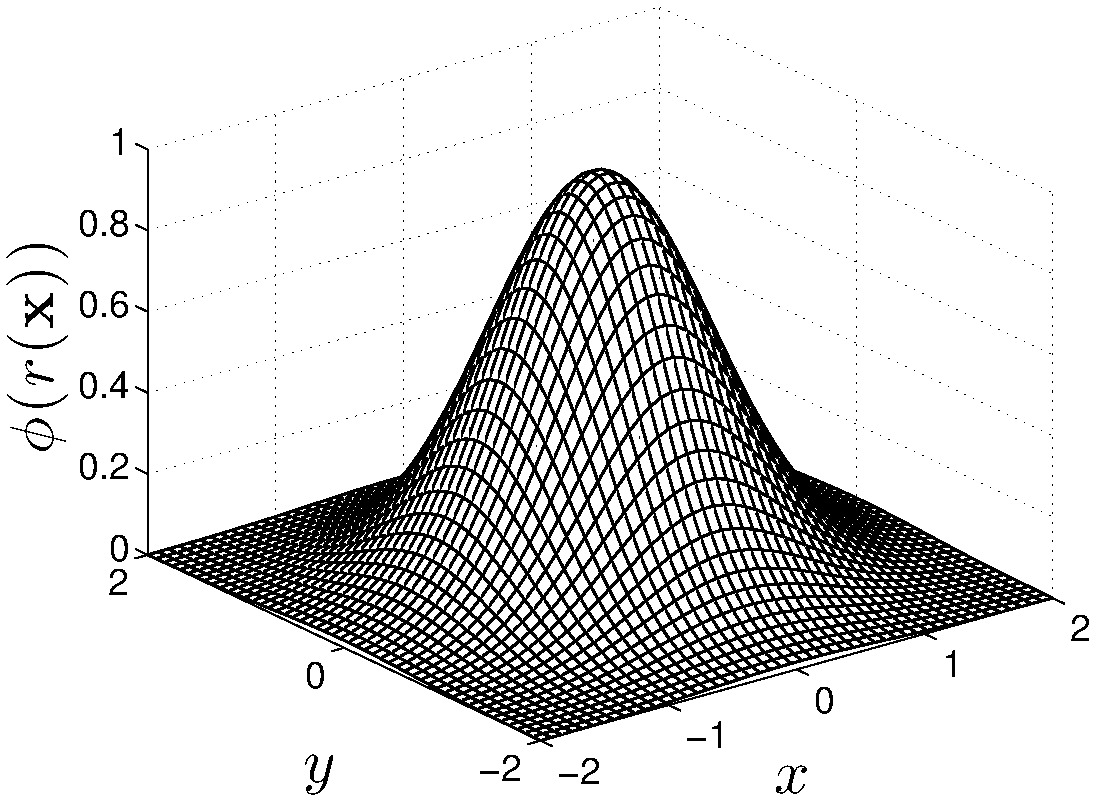
\includegraphics[width=0.25\textwidth]{paper1/figures/ga_rbf2d-eps-converted-to.pdf} }
    \subfigure[Inverse Multiquadric] { 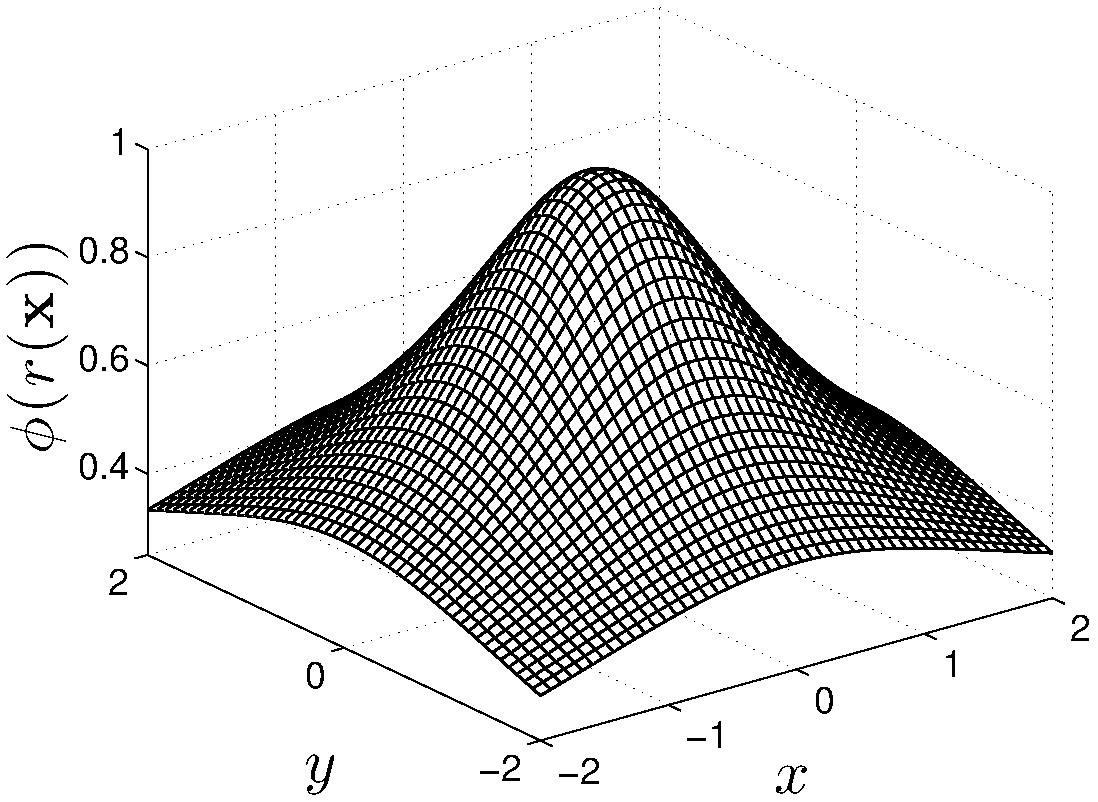
\includegraphics[width=0.25\textwidth]{paper1/figures/imq_rbf2d-eps-converted-to.pdf} }
    \subfigure[Multiquadric] { 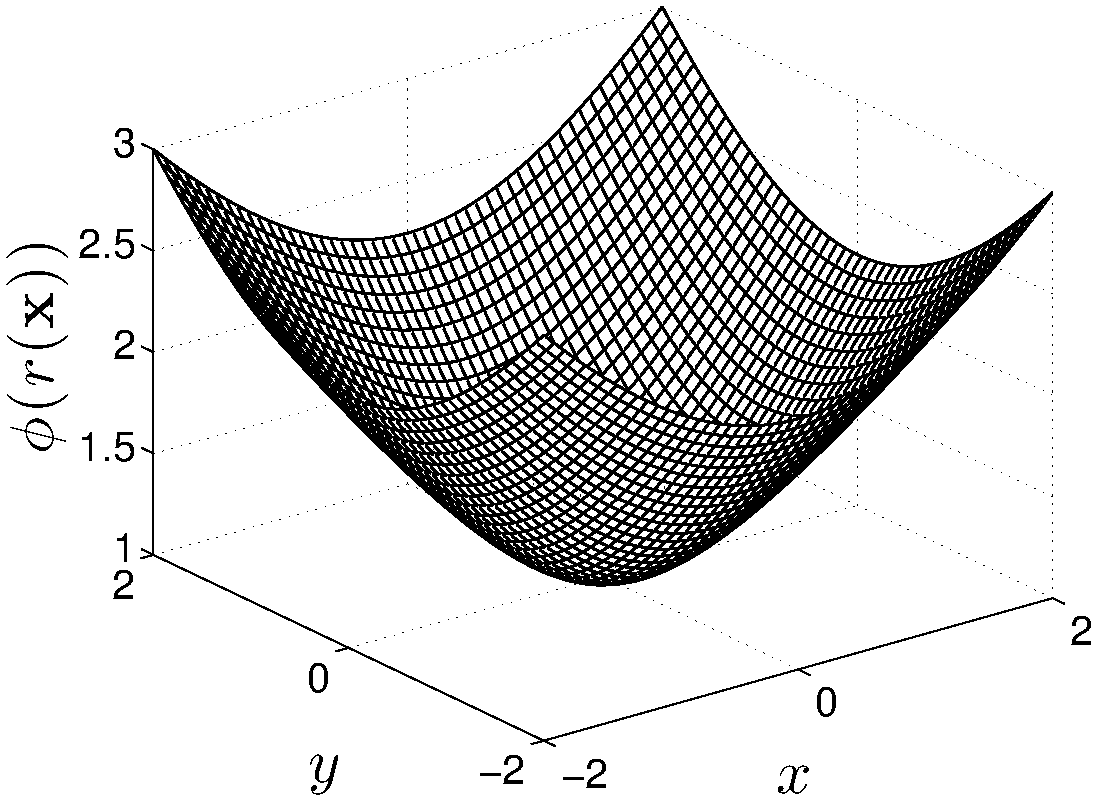
\includegraphics[width=0.25\textwidth]{paper1/figures/mq_rbf2d-eps-converted-to.pdf} }
    \caption{Commonly used RBFs.}
    \label{fig:rbfs}
\end{figure}

Infinitely smooth RBFs depend on a shape or support parameter $\epsilon$ that controls the width of the function. The functional form of the shape function becomes $\phi(\epsilon r)$. Decreasing $\epsilon$ increases the support of the RBF and \ge{}{in most cases,}{2.6} the accuracy of the interpolation, but worsens the conditioning of the RBF interpolation problem \cite{Schaback1995}. Fortunately, recent algorithms such as Contour-Pad\'{e} \cite{Fornberg2004} and RBF-QR \cite{Fornberg2007, Fornberg2011a} allow for numerically stable computation of interpolants in the nearly flat RBF regime (i.e., $\epsilon \rightarrow 0$) where high accuracy has been observed \cite{Larsson2003, Fornberg2008}.

Historically, the most common way to implement RBFs is in a global sense. That is, the value of a function value or any of its derivatives 
at a node location is a linear combination of all the function values over the \textit{entire} domain, just as in a pseudospectral method. If using infinitely smooth RBFs, this leads to exponential convergence of the RBF interpolant for smooth data \eb{}{\cite{Fornberg2005}}{1.3}. %\ge{}{(need reference}{1.3} 
%\st{As discussed in {\cite{FlyerWright09}}, global RBF methods  require a 
%preprocessing stage, executed once, to assemble and solve for the 
%differentiation matrices. This step costs $O(N^3)$ floating point operations,
%where $N$ is the total number of RBFs. 
%The differentiation matrix, DM, is dense and is applied to a vector of 
%function values evaluated at the RBF node centers to obtain an 
%approximation to function derivatives at the RBF node centers. The cost 
%of a derivative calculation is $O(N^2)$. }
\eb{However, this comes at a heavy price in that the matrices are completely full. With $N$ being the total number of nodes, these dense systems scale as $O(N^3)$ operations for calculating the differentiation matrices (DM), a pre-processing step, followed by $O(N^2)$ operations every time-step.}{
As discussed in \cite{FlyerWright09}, global RBF differentiation matrices (DM) are full, requiring $O(N^3)$ floating point operations (FLOPs) to assemble for a given node layout and $O(N^2)$ to time-step.}{}

%$O(N^3)$ floating point operations in pre-processing, where $N$ is the total number of nodes, to assemble and solve a dense linear system that collocates function values at nodes and results in differentiation coefficients. The differentiation coefficients in turn form a dense Differentiation Matrix (DM) that is applied via matrix-vector multiply at every time-step to compute derivatives at a cost of $O(N^2)$ operations. }{1.4}
%%\ge{}{(what matrices?)}{1.4}. 

Alternatively, one can use RBF-generated finite differences (RBF-FD) to introduce sparse DMs (Note: for pure interpolation, compactly supported RBFs can also introduce sparse matrices \cite{Wendland1995}).
RBF-FD was first introduced by Tolstykh in 2000 \cite{Tolstykh2000}, 
but it was the simultaneous, yet independent,
efforts in \cite{Shu2003}, \cite{Tolstykh2003a}, \cite{Wright2003} and \cite{Cecil2004} that gave the method its real start. 
The RBF-FD method is similar in concept to classical 
finite-differences (FD) but differs in that the underlying differentiation 
weights are exact for RBFs rather than polynomials. RBF-FD 
%\ge{}{(yes, spectral and exponential are the same)}{1.5}
share advantages with global RBF methods, 
like the ability to function without an underlying mesh, easily extend to higher dimensions and afford large time steps; however spectral accuracy is lost. 
\ge{Much more advantageous though, is that vast computational speed with still high-order accuracy }{Some of the advantages of RBF-FD 
include high computational speed together with high-order accuracy}{1.6}
(6th to 10th order accuracy is common) and the opportunity 
\ge{to parallelize. }{for parallelization.}{1.6}
As in FD, increasing the stencil size $n$  increases the accuracy of the approximation.
Given $N$ total nodes in the domain (such as on the surface of a sphere), $N$ linear systems, each of size $n \times n$, are solved to calculate the differentiation weights. Since $n \ll N$, the RBF-FD preprocessing complexity is dominated by $O(N)$, much lower than for the global RBF method of $O(N^3)$, with the cost per time step also being $O(N)$. RBF-FD have been successfully employed for a variety of problems including Hamilton-Jacobi equations \cite{Cecil2004}, convection-diffusion problems \cite{Chandhini2007, Stevens2009b},
incompressible Navier-Stokes equations \cite{Shu2003,Chinchapatnam2009}, transport on the sphere \cite{FornbergLehto11}, and the shallow water equations \cite{FlyerLehto11}.

As $N$ grows larger, it behooves us to work on parallel architectures, be it CPUs or GPUs. With regard to the latter, there is some research on leveraging RBFs on GPUs in the fields of visualization \cite{Cuntz2007,Weiler2005},  surface reconstruction \cite{Corrigan2005,Carr2003}, and neural networks \cite{Brandstetter2008}. However, research on the parallelization of RBF algorithms to solve PDEs on multiple CPU/GPU architectures is essentially non-existent. We have found three studies that have addressed this topic, none of which implement RBF-FD but rather take the avenue of domain decomposition for global RBFs (similar to a spectral element approach). In \cite{Divo2007}, Divo and Kassab introduce subdomains with artificial boundaries that are processed independently. Their implementation was designed for a 36 node cluster, but benchmarks and scalability tests are not provided. Kosec and \v{S}arler \cite{Kosec2008} parallelize coupled heat transfer and fluid flow models using OpenMP on a single workstation with one dual-core processor. They achieved a speedup factor of 1.85x over serial execution, although there were
no results from scaling tests. Yokota, Barba and Knepley \cite{Yokota2010} apply a restrictive additive Schwarz domain decomposition to parallelize global RBF interpolation of more then 50 million nodes on 1024 CPU processors. Only Schmidt et al. \cite{Schmidt2009b} have accelerated a global RBF method for PDEs on the GPU. Their MATLAB implementation applies global RBFs to solve the linearized shallow water equations utilizing the AccelerEyes Jacket \cite{JacketGuide2009} library to target a single GPU.

\begin{figure}[t]
    \centering
    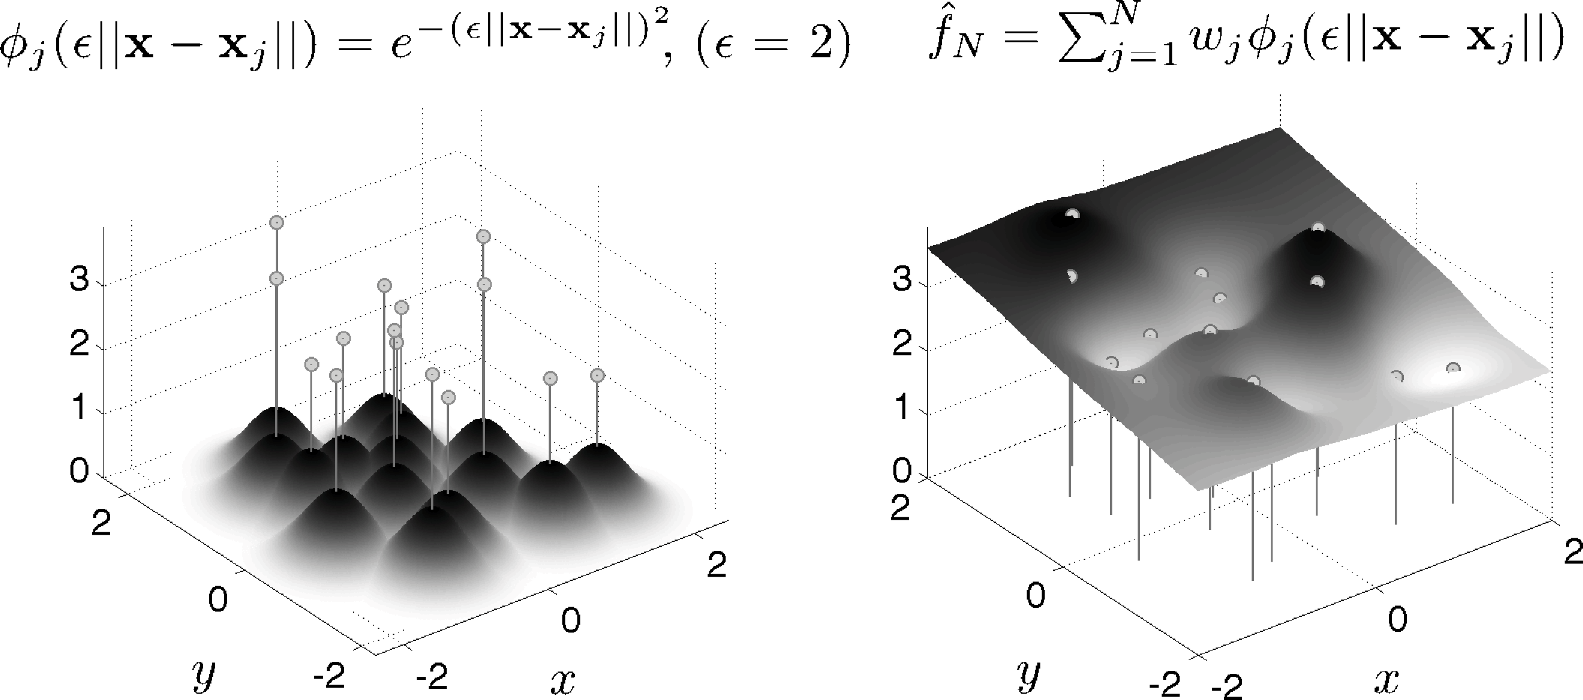
\includegraphics[scale=0.4]{paper1/figures/trimmed_interpolate2D_ga__m_GRAY.pdf}
    \caption{RBF interpolation using 15 translates of the Gaussian RBF with $\epsilon=2$. One RBF is centered at each node in the domain. Linear
    combinations of these produce an interpolant over the domain passing through known function values. }
    \label{fig:rbfInterpolation}
\end{figure}

To our knowledge, this paper presents the first implementation of RBF-FD 
to span multiple CPUs. Each CPU has a corresponding GPU attached to it
in a one-to-one correspondence. We thus also present the first known 
implementation of accelerated RBF-FD on the GPU. Within the scope of this paper we detail our method for spanning RBF-FD across multiple CPU/GPU processors and emphasize numerical validation of the implementation rather than optimization strategies. We will consider optimization in future work. The calculations are performed on Keeneland, a high performance computing installation supported by the National Science Foundation and located at Oak Ridge National Lab. Keeneland currently has 240 CPUs accompanied by 360 NVidia Fermi class GPUs with at least double that number expected by the end of 2012 \cite{Vetter2011}.

The remainder of this paper is organized as follows: Section~\ref{sec:rbffd} introduces RBF-FD via interpolation. Section~\ref{sec:rbffd_gpu} details our parallelization strategies for the Keeneland system, including data partitions that are handled concurrently by different CPU processes and the data-parallel explicit time stepping scheme for the GPU. In Section~\ref{sec:validation}, our implementation is verified against well-known hyperbolic PDE test cases on the sphere, advection of a cosine bell and vortex wrap-up. Finally, performance benchmarks and results are presented in Section~\ref{sec:performance}, followed by conclusions and proposals for future optimization strategies in Section~\ref{sec:conclusion}.

